\documentclass[a4paper, landscape]{article}
\usepackage[utf8]{inputenc}
\usepackage[margin=1.2cm]{geometry}
\usepackage{tikz}
\usetikzlibrary{shapes.geometric, arrows.meta, positioning, fit, backgrounds, calc}

\pagestyle{empty}

\begin{document}

\begin{center}
{\Large\bfseries Scene-Graph Coverage-Driven VLM Testing Framework}\\[4pt]
{\normalsize Complete Pipeline v2 \quad---\quad March 2026}
\end{center}
\vspace{0.5cm}

\centering
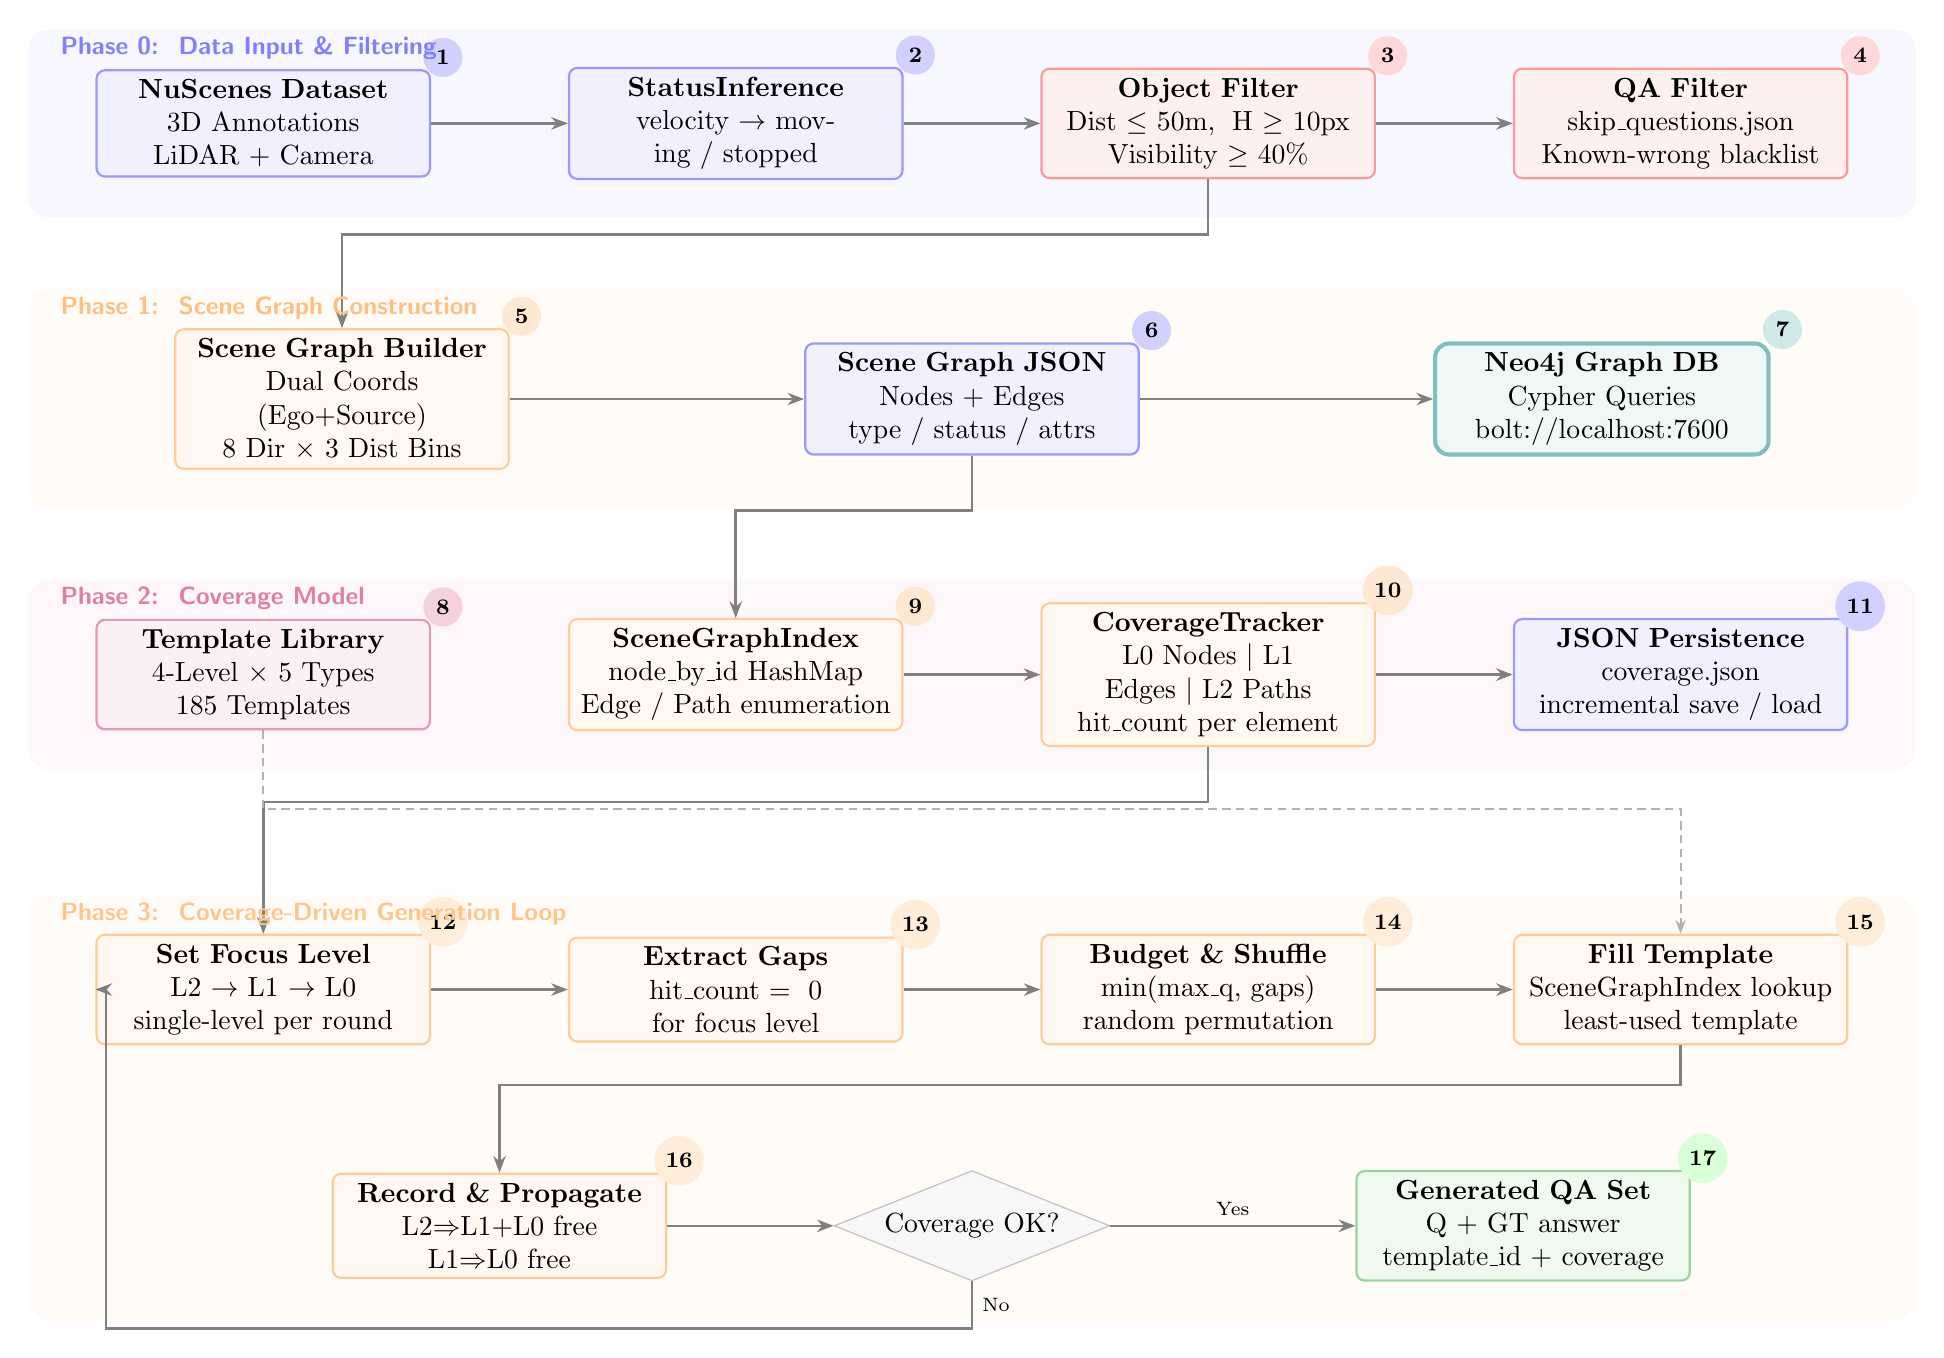
\begin{tikzpicture}[
    % ---- node styles ----
    box/.style={rectangle, draw=#1!40, fill=#1!6,
                text width=4.0cm, text centered,
                minimum height=1.2cm, font=\normalsize,
                rounded corners=3pt, line width=0.8pt},
    box/.default=black,
    dbbox/.style={rectangle, draw=teal!50, fill=teal!6,
                  text width=4.0cm, text centered,
                  minimum height=1.2cm, font=\normalsize,
                  rounded corners=5pt, line width=1.5pt},
    % ---- diamond ----
    chk/.style={diamond, draw=gray!50, fill=gray!6, aspect=2.5,
                font=\normalsize, inner sep=2pt},
    % ---- arrows ----
    arr/.style={-{Stealth[length=6pt]}, line width=0.9pt, draw=black!50},
    darr/.style={-{Stealth[length=5pt]}, line width=0.7pt, densely dashed, draw=black!30},
    % ---- band ----
    band/.style={rounded corners=8pt},
    % ---- circled number ----
    cnum/.style={circle, fill=#1, font=\footnotesize\bfseries,
                 inner sep=2.5pt, text=black},
    cnum/.default=blue!18,
    % ---- layer label ----
    lbl/.style={font=\normalsize\bfseries\sffamily, text=#1!55,
                rotate=90, anchor=south},
    lbl/.default=black,
]

% ============================================================
%  固定band宽度锚点（保证所有层等宽）
% ============================================================
\coordinate (LEFT)  at (-1.5, 0);
\coordinate (RIGHT) at (21.5, 0);

% ============================================================
%  PHASE 0 — Data Input & Filtering
% ============================================================
\node (nuscenes)  [box=blue]  at (1, 0)
    {\textbf{NuScenes Dataset}\\3D Annotations\\LiDAR + Camera};

\node (statusinf) [box=blue]  at (7, 0)
    {\textbf{StatusInference}\\velocity $\to$ moving / stopped};

\node (objfilter) [box=red]   at (13, 0)
    {\textbf{Object Filter}\\Dist $\le$ 50m,\; H $\ge$ 10px\\Visibility $\ge$ 40\%};

\node (qafilter)  [box=red]   at (19, 0)
    {\textbf{QA Filter}\\skip\_questions.json\\Known-wrong blacklist};

% --- Phase 0 arrows ---
\draw [arr] (nuscenes)  -- (statusinf);
\draw [arr] (statusinf) -- (objfilter);
\draw [arr] (objfilter) -- (qafilter);

% --- Phase 0 numbers ---
\node [cnum=blue!18]  at ($(nuscenes.north east) +(0.15,0.15)$) {1};
\node [cnum=blue!18]  at ($(statusinf.north east)+(0.15,0.15)$) {2};
\node [cnum=red!15]   at ($(objfilter.north east)+(0.15,0.15)$) {3};
\node [cnum=red!15]   at ($(qafilter.north east) +(0.15,0.15)$) {4};

% --- Phase 0 background + label ---
\begin{scope}[on background layer]
    \node (bg0) [band, fill=blue!3, inner sep=14pt,
        fit=(LEFT)(RIGHT)(nuscenes)(qafilter)] {};
\end{scope}
\node [anchor=west, font=\small\bfseries\sffamily, text=blue!50]
    at ($(bg0.north west)+(0.3,-0.25)$)
    {Phase 0:\; Data Input \& Filtering};

% ============================================================
%  PHASE 1 — Scene Graph Construction
% ============================================================
\node (sgbuild) [box=orange] at (2, -3.5)
    {\textbf{Scene Graph Builder}\\Dual Coords (Ego+Source)\\8 Dir $\times$ 3 Dist Bins};

\node (sgjson)  [box=blue]   at (10, -3.5)
    {\textbf{Scene Graph JSON}\\Nodes + Edges\\type / status / attrs};

\node (neo4j)   [dbbox]      at (18, -3.5)
    {\textbf{Neo4j Graph DB}\\Cypher Queries\\bolt://localhost:7600};

% --- Phase 0 → 1 arrow (filtered objects go to scene graph) ---
\draw [arr] (objfilter.south) -- ++(0,-0.7) -| (sgbuild.north);

% --- Phase 1 arrows ---
\draw [arr] (sgbuild) -- (sgjson);
\draw [arr] (sgjson)  -- (neo4j);

% --- Phase 1 numbers ---
\node [cnum=orange!18] at ($(sgbuild.north east)+(0.15,0.15)$) {5};
\node [cnum=blue!18]   at ($(sgjson.north east) +(0.15,0.15)$) {6};
\node [cnum=teal!18]   at ($(neo4j.north east)  +(0.15,0.15)$) {7};

% --- Phase 1 background + label ---
\begin{scope}[on background layer]
    \node (bg1) [band, fill=orange!3, inner sep=14pt,
        fit=(LEFT |- sgbuild.north)(RIGHT |- sgbuild.south)(sgbuild)(neo4j)] {};
\end{scope}
\node [anchor=west, font=\small\bfseries\sffamily, text=orange!50]
    at ($(bg1.north west)+(0.3,-0.25)$)
    {Phase 1:\; Scene Graph Construction};

% ============================================================
%  PHASE 2 — Coverage Model
% ============================================================
\node (tmpllib) [box=purple] at (1, -7)
    {\textbf{Template Library}\\4-Level $\times$ 5 Types\\185 Templates};

\node (sgindex) [box=orange] at (7, -7)
    {\textbf{SceneGraphIndex}\\node\_by\_id HashMap\\Edge / Path enumeration};

\node (kvmap)   [box=orange] at (13, -7)
    {\textbf{CoverageTracker}\\L0 Nodes $|$ L1 Edges $|$ L2 Paths\\hit\_count per element};

\node (persist) [box=blue]   at (19, -7)
    {\textbf{JSON Persistence}\\coverage.json\\incremental save / load};

% --- Phase 1 → 2 arrow ---
\draw [arr] (sgjson.south) -- ++(0,-0.7) -| (sgindex.north);

% --- Phase 2 arrows ---
\draw [arr] (sgindex) -- (kvmap);
\draw [arr] (kvmap)   -- (persist);

% --- Phase 2 numbers ---
\node [cnum=purple!18] at ($(tmpllib.north east) +(0.15,0.15)$) {8};
\node [cnum=orange!18] at ($(sgindex.north east) +(0.15,0.15)$) {9};
\node [cnum=orange!18] at ($(kvmap.north east)   +(0.15,0.15)$) {10};
\node [cnum=blue!18]   at ($(persist.north east) +(0.15,0.15)$) {11};

% --- Phase 2 background + label ---
\begin{scope}[on background layer]
    \node (bg2) [band, fill=purple!3, inner sep=14pt,
        fit=(LEFT |- tmpllib.north)(RIGHT |- tmpllib.south)(tmpllib)(persist)] {};
\end{scope}
\node [anchor=west, font=\small\bfseries\sffamily, text=purple!50]
    at ($(bg2.north west)+(0.3,-0.25)$)
    {Phase 2:\; Coverage Model};

% ============================================================
%  PHASE 3 — Coverage-Driven Generation Loop
% ============================================================
\node (focus)  [box=orange] at (1, -11)
    {\textbf{Set Focus Level}\\L2 $\to$ L1 $\to$ L0\\single-level per round};

\node (gaps)   [box=orange] at (7, -11)
    {\textbf{Extract Gaps}\\hit\_count $= 0$\\for focus level};

\node (budget) [box=orange] at (13, -11)
    {\textbf{Budget \& Shuffle}\\min(max\_q, gaps)\\random permutation};

\node (gen)    [box=orange] at (19, -11)
    {\textbf{Fill Template}\\SceneGraphIndex lookup\\least-used template};

\node (record) [box=orange] at (4, -14)
    {\textbf{Record \& Propagate}\\L2$\Rightarrow$L1+L0 free\\L1$\Rightarrow$L0 free};

\node (chkdone) [chk] at (10, -14)
    {Coverage OK?};

\node (qaout)  [box=green!60!black] at (17, -14)
    {\textbf{Generated QA Set}\\Q + GT answer\\template\_id + coverage};

% --- Phase 2 → 3 arrows ---
\draw [arr] (kvmap.south) -- ++(0,-0.7) -| (focus.north);

% --- Phase 3 arrows: linear flow ---
\draw [arr] (focus)  -- (gaps);
\draw [arr] (gaps)   -- (budget);
\draw [arr] (budget) -- (gen);
\draw [arr] (gen.south) -- ++(0,-0.5) -| (record.north);
\draw [arr] (record) -- (chkdone);

% --- loop back (outside path: down → left → up → right into focus) ---
\draw [arr] (chkdone.south) -- ++(0,-0.6)
    node[pos=0.5, right, font=\scriptsize]{No}
    -| (-1, -14.6) -- (-1, -11) -- (focus.west);

% --- QA output ---
\draw [arr] (chkdone.east) -- node[above, font=\scriptsize]{Yes} (qaout.west);

% --- Template Library feeds into Fill Template (dashed) ---
\draw [darr] (tmpllib.south) -- ++(0,-1.0) -| (gen.north);

% --- Phase 3 numbers ---
\node [cnum=orange!15] at ($(focus.north east) +(0.15,0.15)$) {12};
\node [cnum=orange!15] at ($(gaps.north east)  +(0.15,0.15)$) {13};
\node [cnum=orange!15] at ($(budget.north east)+(0.15,0.15)$) {14};
\node [cnum=orange!15] at ($(gen.north east)   +(0.15,0.15)$) {15};
\node [cnum=orange!15] at ($(record.north east)+(0.15,0.15)$) {16};
\node [cnum=green!15]  at ($(qaout.north east) +(0.15,0.15)$) {17};

% --- Phase 3 background + label ---
\begin{scope}[on background layer]
    \node (bg3) [band, fill=orange!3, inner sep=14pt,
        fit=(LEFT |- focus.north)(RIGHT |- record.south)
            (focus)(gen)(record)(chkdone)(qaout)] {};
\end{scope}
\node [anchor=west, font=\small\bfseries\sffamily, text=orange!45]
    at ($(bg3.north west)+(0.3,-0.25)$)
    {Phase 3:\; Coverage-Driven Generation Loop};

% ============================================================
%  下方留白（本页到此结束）
% ============================================================

\end{tikzpicture}

\newpage

% ====================================================================
%  PAGE 2 — Phase 4 + Phase 5
% ====================================================================
\begin{center}
{\Large\bfseries Scene-Graph Coverage-Driven VLM Testing Framework}\\[4pt]
{\normalsize Pipeline (continued) — Phase 4 \& 5}
\end{center}
\vspace{0.5cm}

\centering
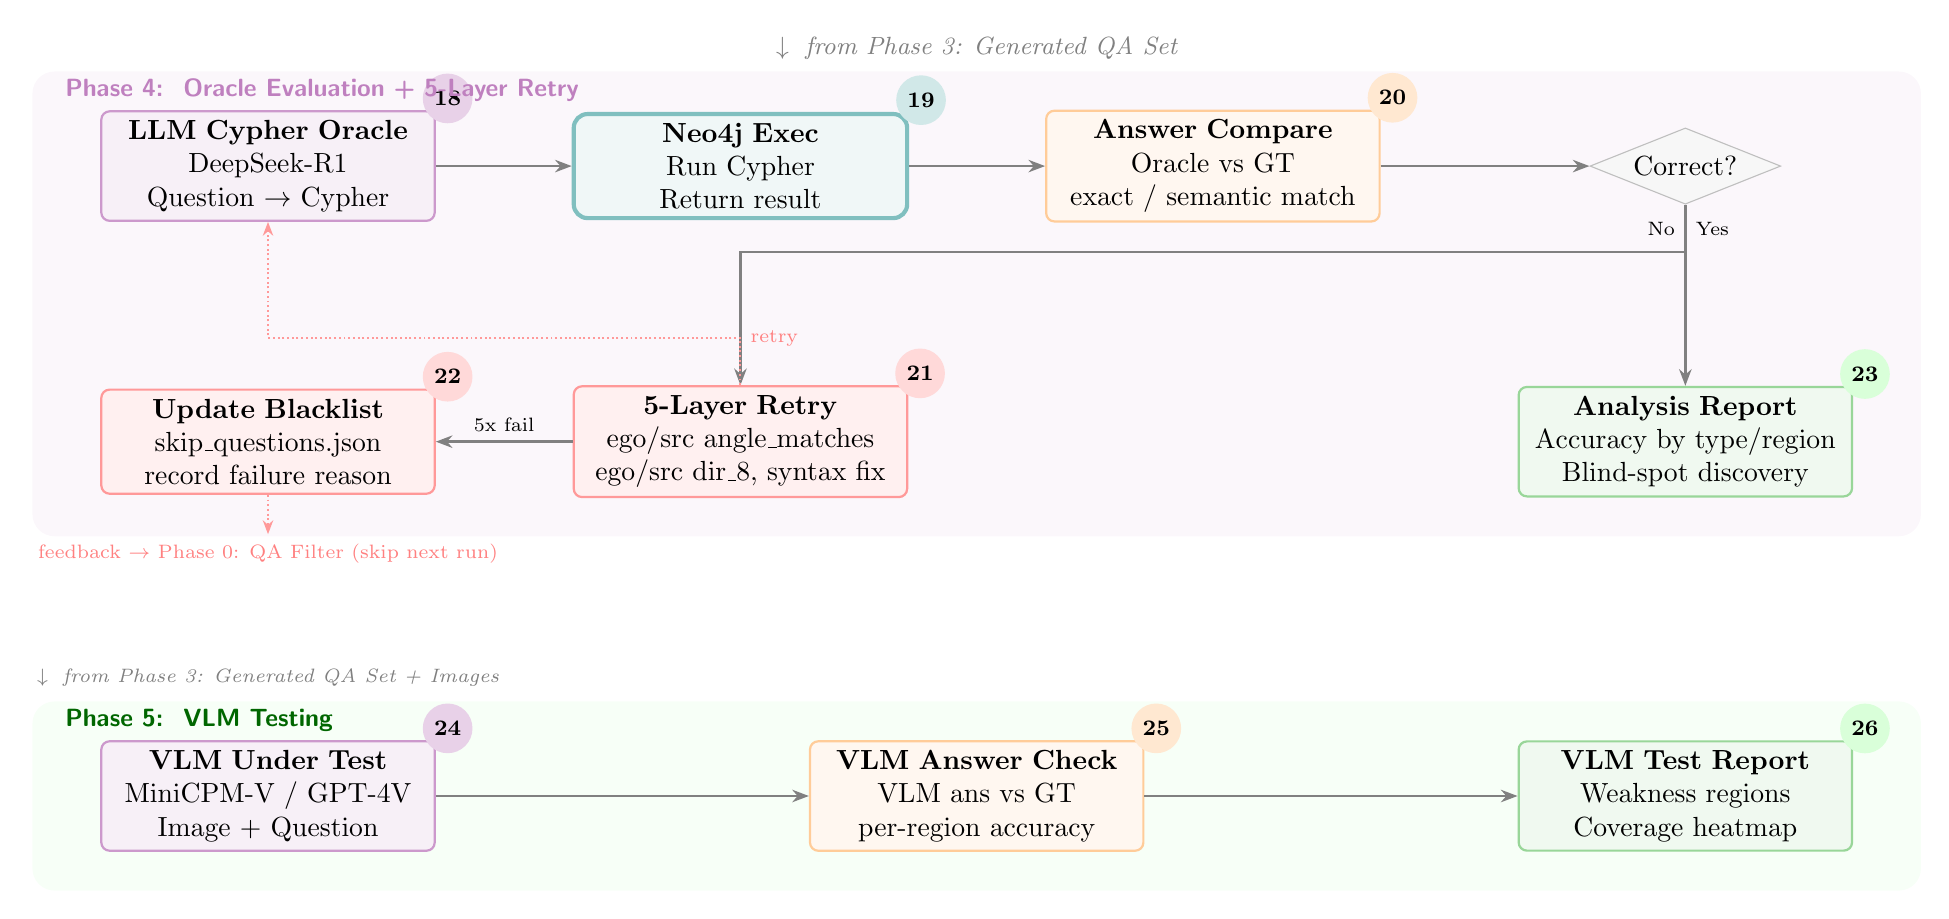
\begin{tikzpicture}[
    box/.style={rectangle, draw=#1!40, fill=#1!6,
                text width=4.0cm, text centered,
                minimum height=1.2cm, font=\normalsize,
                rounded corners=3pt, line width=0.8pt},
    box/.default=black,
    dbbox/.style={rectangle, draw=teal!50, fill=teal!6,
                  text width=4.0cm, text centered,
                  minimum height=1.2cm, font=\normalsize,
                  rounded corners=5pt, line width=1.5pt},
    chk/.style={diamond, draw=gray!50, fill=gray!6, aspect=2.5,
                font=\normalsize, inner sep=2pt},
    arr/.style={-{Stealth[length=6pt]}, line width=0.9pt, draw=black!50},
    darr/.style={-{Stealth[length=5pt]}, line width=0.7pt, densely dashed, draw=black!30},
    retarr/.style={-{Stealth[length=5pt]}, line width=0.7pt, densely dotted, draw=red!40},
    band/.style={rounded corners=8pt},
    cnum/.style={circle, fill=#1, font=\footnotesize\bfseries,
                 inner sep=2.5pt, text=black},
    cnum/.default=blue!18,
]

% --- 等宽锚点 ---
\coordinate (LEFT)  at (-1.5, 0);
\coordinate (RIGHT) at (21.5, 0);

% --- 入口提示：来自上页 Generated QA Set ---
\node [font=\small\itshape, text=gray] at (10, 1.5)
    {$\downarrow$\; from Phase 3: Generated QA Set};

% ============================================================
%  PHASE 4 — Oracle Evaluation + 5-Layer Retry
% ============================================================
\node (llmoracle) [box=violet] at (1, 0)
    {\textbf{LLM Cypher Oracle}\\DeepSeek-R1\\Question $\to$ Cypher};

\node (neo4jq) [dbbox] at (7, 0)
    {\textbf{Neo4j Exec}\\Run Cypher\\Return result};

\node (compare) [box=orange] at (13, 0)
    {\textbf{Answer Compare}\\Oracle vs GT\\exact / semantic match};

\node (retrychk) [chk] at (19, 0)
    {Correct?};

% --- row 2 ---
\node (retrybox) [box=red] at (7, -3.5)
    {\textbf{5-Layer Retry}\\ego/src angle\_matches\\ego/src dir\_8, syntax fix};

\node (blacklist) [box=red] at (1, -3.5)
    {\textbf{Update Blacklist}\\skip\_questions.json\\record failure reason};

\node (result) [box=green!60!black] at (19, -3.5)
    {\textbf{Analysis Report}\\Accuracy by type/region\\Blind-spot discovery};

% --- Phase 4 arrows ---
\draw [arr] (llmoracle) -- (neo4jq);
\draw [arr] (neo4jq) -- (compare);
\draw [arr] (compare) -- (retrychk);

% Correct → Analysis Report
\draw [arr] (retrychk.south) -- ++(0,-0.6)
    node[pos=0.5, right, font=\scriptsize]{Yes}
    -| (result.north);

% Incorrect → Retry
\draw [arr] (retrychk.south) -- ++(0,-0.6)
    node[pos=0.5, left, font=\scriptsize]{No}
    -| (retrybox.north);

% Retry → back to LLM Oracle (goes up from retry box)
\draw [retarr] (retrybox.north) -- ++(0,0.6) -| (llmoracle.south)
    node[pos=0.0, right, font=\scriptsize, text=red!50]{retry};

% Exhausted → Blacklist
\draw [arr] (retrybox) -- node[above, font=\scriptsize]{5x fail} (blacklist);

% --- Phase 4 numbers ---
\node [cnum=violet!18] at ($(llmoracle.north east)+(0.15,0.15)$) {18};
\node [cnum=teal!18]   at ($(neo4jq.north east)   +(0.15,0.15)$) {19};
\node [cnum=orange!18] at ($(compare.north east)  +(0.15,0.15)$) {20};
\node [cnum=red!15]    at ($(retrybox.north east) +(0.15,0.15)$) {21};
\node [cnum=red!15]    at ($(blacklist.north east) +(0.15,0.15)$) {22};
\node [cnum=green!15]  at ($(result.north east)   +(0.15,0.15)$) {23};

% --- Phase 4 background + label ---
\begin{scope}[on background layer]
    \node (bg4) [band, fill=violet!3, inner sep=14pt,
        fit=(LEFT)(RIGHT)(llmoracle)(retrychk)(blacklist)(result)] {};
\end{scope}
\node [anchor=west, font=\small\bfseries\sffamily, text=violet!50]
    at ($(bg4.north west)+(0.3,-0.25)$)
    {Phase 4:\; Oracle Evaluation + 5-Layer Retry};

% ============================================================
%  Blacklist feedback annotation
% ============================================================
\draw [retarr] (blacklist.south) -- ++(0,-0.5)
    node[below, font=\scriptsize, text=red!50]
    {feedback $\to$ Phase 0: QA Filter (skip next run)};

% ============================================================
%  PHASE 5 — VLM Testing
% ============================================================
\node (vlm) [box=violet] at (1, -8)
    {\textbf{VLM Under Test}\\MiniCPM-V / GPT-4V\\Image + Question};

\node (vlmcmp) [box=orange] at (10, -8)
    {\textbf{VLM Answer Check}\\VLM ans vs GT\\per-region accuracy};

\node (vlmresult) [box=green!60!black] at (19, -8)
    {\textbf{VLM Test Report}\\Weakness regions\\Coverage heatmap};

% --- 入口提示：来自 Generated QA Set ---
\node [font=\scriptsize\itshape, text=gray] at (1, -6.5)
    {$\downarrow$\; from Phase 3: Generated QA Set + Images};

% --- Phase 5 arrows ---
\draw [arr] (vlm) -- (vlmcmp);
\draw [arr] (vlmcmp) -- (vlmresult);

% --- Phase 5 numbers ---
\node [cnum=violet!18]  at ($(vlm.north east)      +(0.15,0.15)$) {24};
\node [cnum=orange!18]  at ($(vlmcmp.north east)   +(0.15,0.15)$) {25};
\node [cnum=green!15]   at ($(vlmresult.north east)+(0.15,0.15)$) {26};

% --- Phase 5 background + label ---
\begin{scope}[on background layer]
    \node (bg5) [band, fill=green!3, inner sep=14pt,
        fit=(LEFT |- vlm.north)(RIGHT |- vlm.south)(vlm)(vlmresult)] {};
\end{scope}
\node [anchor=west, font=\small\bfseries\sffamily, text=green!40!black]
    at ($(bg5.north west)+(0.3,-0.25)$)
    {Phase 5:\; VLM Testing};

\end{tikzpicture}

\end{document}
